\documentclass[11pt]{article}
\usepackage{amsmath, amssymb, amsfonts, amsthm}
\usepackage{geometry}
\geometry{letterpaper, margin=0.5in}
\usepackage{booktabs}
\usepackage{tikz}
\usepackage{hyperref}
\usepackage{makecell}
\usepackage{longtable}s

\newcommand{\noi}{\noindent}
\newcommand{\tbf}{\textbf}
\newcommand{\lb}{\left\{}
\newcommand{\rb}{\right\}}
\newcommand{\Z}{\mathbb{Z}}

\theoremstyle{definition} 
\newtheorem{definition}{Definition}[section]

\newif\ifrootsystemirreducible
\rootsystemirreducibletrue

\newif\ifrootsystemreduced
\rootsystemreducedtrue

\newif\ifsummablepairs
\summablepairstrue

\title{Pinned group summary: SL-n3}
\author{Pinning-Sympy automated output}
\date{\today}

\begin{document}

\maketitle
\tableofcontents

\newpage

\section{Basic group attributes}

\def\arraystretch{1.2}
\begin{tabular}{|l|l|}
	\hline
    Group & SL-n3 \\
	\hline
    Matrix size & $3 \times 3$ \\
	\hline
    Rank & $2$ \\
	\hline
	Defining equations & $\operatorname{det}(X)=1$ \\
	\hline
\end{tabular}
\def\arraystretch{1}



\subsection{Lie algebra}

The defining equations for the Lie algebra are: $\operatorname{tr}(X)=0$

\noi A generic element of the Lie algebra is:
\[
\left[\begin{matrix}x_{0 0} & x_{0 1} & x_{0 2}\\x_{1 0} & x_{1 1} & x_{1 2}\\x_{2 0} & x_{2 1} & - x_{0 0} - x_{1 1}\end{matrix}\right]
\]

\subsection{Torus}

The torus has rank $2$. A generic element of the torus is
\[
\left[\begin{matrix}t_{0} & 0 & 0\\0 & t_{1} & 0\\0 & 0 & \frac{1}{t_{0} t_{1}}\end{matrix}\right]
\]
The rows of the matrix below are trivial characters:
\[
\left[\begin{matrix}1 & 1 & 1\end{matrix}\right]
\]

\newpage
\section{Root system}

\begin{tabular}{|l|l|}
	\hline
    Dynkin type & $A_2$ \\
	\hline
    Irreducible & True \\
	\hline
    Reduced & True \\
	\hline
	Simply laced & True \\
	\hline
	Number of roots & $6$ \\
	\hline
\end{tabular}

\subsection{Dynkin diagram}

\ifrootsystemirreducible
The root system is irreducible and has Dynkin diagram:
\else
The root system is reducible with RootSystemComponentsPlaceholder components. The Dynkin diagrams of the respective components are:
\fi

\begin{center}
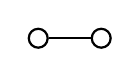
\begin{tikzpicture}[scale=1, baseline=(current bounding box.center),
    node/.style={circle, draw, minimum size=0.24cm, inner sep=0pt, thick, fill=white},
    filled/.style={circle, draw, minimum size=0.24cm, inner sep=0pt, thick, fill=black}
]
  \node[node] (v1) at (0.0, 0) {};
  \node[node] (v2) at (0.8, 0) {};
  \draw[thick] (v1) -- (v2);
\end{tikzpicture}
\end{center}

\subsection{Cartan matrix}

\ifrootsystemirreducible
The root system is irreducible and has Cartan matrix:
\else
The root system is reducible with RootSystemComponentsPlaceholder components. The Cartan matrices of the respective components are:
\fi

\[
\left[\begin{matrix}2 & -1\\-1 & 2\end{matrix}\right]
\]

\subsection{Roots}

\begin{definition}
A root $\alpha \in \Phi$ is \tbf{multipliable} if $2\alpha \in \Phi$.
\end{definition}

\noi \begin{tabular}{|l|c|c|c|c|}
    \hline
    \textbf{Root} & \textbf{Squared norm} & \textbf{Simple} & \textbf{Sign} & \textbf{Multipliable} \\
    \hline
    $\left( 0, \  1, \  -1\right)$ & $2$ & Yes & $+$ & No \\
    \hline
    $\left( 1, \  -1, \  0\right)$ & $2$ & Yes & $+$ & No \\
    \hline
    $\left( 1, \  0, \  -1\right)$ & $2$ & No & $+$ & No \\
    \hline
    $\left( -1, \  0, \  1\right)$ & $2$ & No & $-$ & No \\
    \hline
    $\left( -1, \  1, \  0\right)$ & $2$ & No & $-$ & No \\
    \hline
    $\left( 0, \  -1, \  1\right)$ & $2$ & No & $-$ & No \\
    \hline
\end{tabular}


\subsection{Coroots}

\begin{tabular}{|l|l|}
    \hline
    \textbf{Root} & \textbf{Coroot} \\
    \hline
    $\left( -1, \  0, \  1\right)$ & $\left( -1, \  0, \  1\right)$ \\
    \hline
    $\left( -1, \  1, \  0\right)$ & $\left( -1, \  1, \  0\right)$ \\
    \hline
    $\left( 0, \  -1, \  1\right)$ & $\left( 0, \  -1, \  1\right)$ \\
    \hline
    $\left( 0, \  1, \  -1\right)$ & $\left( 0, \  1, \  -1\right)$ \\
    \hline
    $\left( 1, \  -1, \  0\right)$ & $\left( 1, \  -1, \  0\right)$ \\
    \hline
    $\left( 1, \  0, \  -1\right)$ & $\left( 1, \  0, \  -1\right)$ \\
    \hline
\end{tabular}


\ifsummablepairs
\subsection{Linear combinations of roots}

\begin{definition}
For two roots $\alpha, \beta$ in a root system $\Phi$, the set of positive integral linear combinations of $\alpha, \beta$ that are also roots is denoted
\(
	(\alpha, \beta) = \{ i \alpha + j \beta \in \Phi : i, j \in \mathbb{Z}_{\ge 1} \}
\).
\end{definition}

\noi \noindent \begin{longtable}{|l|l|c|}
    \hline
    $\alpha$ & $\beta$ & Pairs $(i,j)$ \\
    \hline
    \endhead
    $\left( -1, \  0, \  1\right)$ & $\left( 0, \  1, \  -1\right)$ & $(1,1)$ \\
    \hline
    $\left( -1, \  0, \  1\right)$ & $\left( 1, \  -1, \  0\right)$ & $(1,1)$ \\
    \hline
    $\left( -1, \  1, \  0\right)$ & $\left( 0, \  -1, \  1\right)$ & $(1,1)$ \\
    \hline
    $\left( -1, \  1, \  0\right)$ & $\left( 1, \  0, \  -1\right)$ & $(1,1)$ \\
    \hline
    $\left( 0, \  -1, \  1\right)$ & $\left( 1, \  0, \  -1\right)$ & $(1,1)$ \\
    \hline
    $\left( 0, \  1, \  -1\right)$ & $\left( 1, \  -1, \  0\right)$ & $(1,1)$ \\
    \hline
\end{longtable}

\fi

\newpage
\section{Root spaces}

\subsection{Dimensions}

The table below lists each root along with the dimension of the associated root space (and root subgroup).

\bigskip

\noindent \begin{tabular}{|l|c|}
    \hline
    \textbf{Root ($\alpha$)} & \textbf{Dimension of root space ($d_{\alpha}$)} \\
    \hline
    $\left( -1, \  0, \  1\right)$ & 1 \\
    \hline
    $\left( -1, \  1, \  0\right)$ & 1 \\
    \hline
    $\left( 0, \  -1, \  1\right)$ & 1 \\
    \hline
    $\left( 0, \  1, \  -1\right)$ & 1 \\
    \hline
    $\left( 1, \  -1, \  0\right)$ & 1 \\
    \hline
    $\left( 1, \  0, \  -1\right)$ & 1 \\
    \hline
\end{tabular}


\subsection{Root space table}

\noi The table below lists each root along with a generic element of the associated root space (inside the Lie algebra). Include a definition here? INCOMPLETE

\bigskip

\noindent \begin{longtable}{|l|c|}
    \hline
    \textbf{Root} & \textbf{Generic element of root space} \\
    \hline
    \endhead
    $\left( -1, \  0, \  1\right)$ & ${\left[\begin{matrix}0 & 0 & 0\\0 & 0 & 0\\u_{0} & 0 & 0\end{matrix}\right]}$ \\
    \hline
    $\left( -1, \  1, \  0\right)$ & ${\left[\begin{matrix}0 & 0 & 0\\u_{0} & 0 & 0\\0 & 0 & 0\end{matrix}\right]}$ \\
    \hline
    $\left( 0, \  -1, \  1\right)$ & ${\left[\begin{matrix}0 & 0 & 0\\0 & 0 & 0\\0 & u_{0} & 0\end{matrix}\right]}$ \\
    \hline
    $\left( 0, \  1, \  -1\right)$ & ${\left[\begin{matrix}0 & 0 & 0\\0 & 0 & u_{0}\\0 & 0 & 0\end{matrix}\right]}$ \\
    \hline
    $\left( 1, \  -1, \  0\right)$ & ${\left[\begin{matrix}0 & u_{0} & 0\\0 & 0 & 0\\0 & 0 & 0\end{matrix}\right]}$ \\
    \hline
    $\left( 1, \  0, \  -1\right)$ & ${\left[\begin{matrix}0 & 0 & u_{0}\\0 & 0 & 0\\0 & 0 & 0\end{matrix}\right]}$ \\
    \hline
\end{longtable}


\newpage
\section{Root subgroups}

\subsection{Root subgroup table}

\noi The table below lists each root along with a generic element of the associated root subgroup.

\bigskip

\noindent \begin{longtable}{|l|c|}
    \hline
    \textbf{Root} & \textbf{Generic element of root subgroup} \\
    \hline
    \endhead
    $\left( -1, \  0, \  1\right)$ & ${\left[\begin{matrix}1 & 0 & 0\\0 & 1 & 0\\u_{0} & 0 & 1\end{matrix}\right]}$ \\
    \hline
    $\left( -1, \  1, \  0\right)$ & ${\left[\begin{matrix}1 & 0 & 0\\u_{0} & 1 & 0\\0 & 0 & 1\end{matrix}\right]}$ \\
    \hline
    $\left( 0, \  -1, \  1\right)$ & ${\left[\begin{matrix}1 & 0 & 0\\0 & 1 & 0\\0 & u_{0} & 1\end{matrix}\right]}$ \\
    \hline
    $\left( 0, \  1, \  -1\right)$ & ${\left[\begin{matrix}1 & 0 & 0\\0 & 1 & u_{0}\\0 & 0 & 1\end{matrix}\right]}$ \\
    \hline
    $\left( 1, \  -1, \  0\right)$ & ${\left[\begin{matrix}1 & u_{0} & 0\\0 & 1 & 0\\0 & 0 & 1\end{matrix}\right]}$ \\
    \hline
    $\left( 1, \  0, \  -1\right)$ & ${\left[\begin{matrix}1 & 0 & u_{0}\\0 & 1 & 0\\0 & 0 & 1\end{matrix}\right]}$ \\
    \hline
\end{longtable}


\subsection{Homomorphism property}

\noi For each root $\alpha \in \Phi$, the associated root subgroup map $X_\alpha:V_\alpha \to G$ is a pseudo-homomorphism with respect to the additive structure on $V_\alpha$ and the group operation (i.e. matrix multiplication) in $G$. That is, for any $u,v \in V_\alpha$,
\begin{equation}
\label{pseudo homomorphism}
	X_\alpha(u) \cdot X_\alpha(v) = X_\alpha(u+v) \cdot \prod_{\substack{i > 1 \\ i \alpha \in \Phi}} X_{i \alpha} \Big( q^i_\alpha(u,v) \Big)
\end{equation}
for some homogeneous polynomial maps $q^i_\alpha:V_\alpha \times V_\alpha \to V_{i \alpha}$. Thus $X_\alpha$ is a group homomorphism if and only the product on the right hand side reduces to 1. The quantities $q^i_\alpha(u,v)$ are called \tbf{homomorphism defect coefficients}. For any root $\alpha$ of a root system $\Phi$ of any group considered in the Pinning-Sympy package, the set
\[
	\lb i \alpha \in \Phi : i \in \Z_{\ge 2} \rb
\]
is either empty or a singleton set consisting of $\lb 2 \alpha \rb$. The non-empty case only arises when $\Phi$ is a non-reduced root system (of Dynkin type $\mathsf{BC}$), and when $\alpha$ is a multipliable root. 

\ifrootsystemreduced
Since the root system for this group is reduced, there are no multipliable roots and the product is always empty, hence each $X_\alpha$ is a group homomorphism there are no homomorphism defect coefficients.
\else
The table below lists all multipliable roots and the associated homomorphism defect.

\bigskip

HomomorphismDefectTablePlaceholder

\bigskip

\noi Below is an explicit formulation of the homomorphism/pseudo-homomorphism identities.

\bigskip

HomomorphismDefectIdentitiesPlaceholder
\fi

\ifsummablepairs
\newpage
\section{Commutators}

The Steinberg/Chevalley commutator formula says that for two roots $\alpha, \beta \in \Phi$, the commutator of two root group elements $X_\alpha(u)$ and $X_\beta(v)$ is controlled by the structure of $\Phi$, in particular by which positive integer linear combinations $i\alpha + j\beta$ are elements of $\Phi$. Recall that
\[
	(\alpha, \beta) = \lb i \alpha + j\beta \in \Phi : i, j \in \Z_{\ge 1} \rb
\]
Specifically, we have the commutator formula
\[
	\Big[ X_\alpha(u), X_\beta(v) \Big] = \prod_{(\alpha, \beta)} X_{i\alpha + j\beta} \Big( N_{ij}^{\alpha \beta}(u,v) \Big)
\]
for some homogeneous polynomial functions $N_{ij}^{\alpha \beta}:V_{\alpha} \times V_{\beta} \to V_{i\alpha+j\beta}$. We repeat here the table of linear combinations of roots. The quantity $N_{ij}^{\alpha \beta}(u,v)$ is called a \tbf{commutator coefficient}. The table below gives these coefficients.

\bigskip

\noi \noindent \begin{longtable}{|l|l|c|c|l|c|}
    \hline
    $\alpha$ & $\beta$ & $i$ & $j$ &  $i\alpha + j\beta$ & $N_{ij}^{\alpha\beta}(u,v)$ \\
    \hline
    \endhead
    $\left( -1, \  0, \  1\right)$ & $\left( 0, \  1, \  -1\right)$ & 1 & 1 & $\left( -1, \  1, \  0\right)$ & $- u_{0} v_{0}$ \\
    \hline
    $\left( -1, \  0, \  1\right)$ & $\left( 1, \  -1, \  0\right)$ & 1 & 1 & $\left( 0, \  -1, \  1\right)$ & $u_{0} v_{0}$ \\
    \hline
    $\left( -1, \  1, \  0\right)$ & $\left( 0, \  -1, \  1\right)$ & 1 & 1 & $\left( -1, \  0, \  1\right)$ & $- u_{0} v_{0}$ \\
    \hline
    $\left( -1, \  1, \  0\right)$ & $\left( 1, \  0, \  -1\right)$ & 1 & 1 & $\left( 0, \  1, \  -1\right)$ & $u_{0} v_{0}$ \\
    \hline
    $\left( 0, \  -1, \  1\right)$ & $\left( -1, \  1, \  0\right)$ & 1 & 1 & $\left( -1, \  0, \  1\right)$ & $u_{0} v_{0}$ \\
    \hline
    $\left( 0, \  -1, \  1\right)$ & $\left( 1, \  0, \  -1\right)$ & 1 & 1 & $\left( 1, \  -1, \  0\right)$ & $- u_{0} v_{0}$ \\
    \hline
    $\left( 0, \  1, \  -1\right)$ & $\left( -1, \  0, \  1\right)$ & 1 & 1 & $\left( -1, \  1, \  0\right)$ & $u_{0} v_{0}$ \\
    \hline
    $\left( 0, \  1, \  -1\right)$ & $\left( 1, \  -1, \  0\right)$ & 1 & 1 & $\left( 1, \  0, \  -1\right)$ & $- u_{0} v_{0}$ \\
    \hline
    $\left( 1, \  -1, \  0\right)$ & $\left( -1, \  0, \  1\right)$ & 1 & 1 & $\left( 0, \  -1, \  1\right)$ & $- u_{0} v_{0}$ \\
    \hline
    $\left( 1, \  -1, \  0\right)$ & $\left( 0, \  1, \  -1\right)$ & 1 & 1 & $\left( 1, \  0, \  -1\right)$ & $u_{0} v_{0}$ \\
    \hline
    $\left( 1, \  0, \  -1\right)$ & $\left( -1, \  1, \  0\right)$ & 1 & 1 & $\left( 0, \  1, \  -1\right)$ & $- u_{0} v_{0}$ \\
    \hline
    $\left( 1, \  0, \  -1\right)$ & $\left( 0, \  -1, \  1\right)$ & 1 & 1 & $\left( 1, \  -1, \  0\right)$ & $u_{0} v_{0}$ \\
    \hline
\end{longtable}


\subsection{Commutator identities}

\noi Below is an explicit formulation of the commutator formula identities.

\bigskip

\noi CommutatorIdentitiesPlaceholder
\fi

\newpage
\section{Weyl group}

\noi Background theoretical info on Weyl group, especially as realized inside the group, including info on conjugation between root subgroups INCOMPLETE

\subsection{Weyl group elements}

\noi The table below lists roots along with an associated Weyl group element.

\bigskip

\noi \noindent \begin{longtable}{|l|c|}
    \hline
    \textbf{Root} & \textbf{Weyl group element} \\
    \hline
    \endhead
    $\left( -1, \  0, \  1\right)$ & ${\left[\begin{matrix}0 & 0 & 1\\0 & 1 & 0\\-1 & 0 & 0\end{matrix}\right]}$ \\
    \hline
    $\left( -1, \  1, \  0\right)$ & ${\left[\begin{matrix}0 & 1 & 0\\-1 & 0 & 0\\0 & 0 & 1\end{matrix}\right]}$ \\
    \hline
    $\left( 0, \  -1, \  1\right)$ & ${\left[\begin{matrix}1 & 0 & 0\\0 & 0 & -1\\0 & 1 & 0\end{matrix}\right]}$ \\
    \hline
    $\left( 0, \  1, \  -1\right)$ & ${\left[\begin{matrix}1 & 0 & 0\\0 & 0 & -1\\0 & 1 & 0\end{matrix}\right]}$ \\
    \hline
    $\left( 1, \  -1, \  0\right)$ & ${\left[\begin{matrix}0 & 1 & 0\\-1 & 0 & 0\\0 & 0 & 1\end{matrix}\right]}$ \\
    \hline
    $\left( 1, \  0, \  -1\right)$ & ${\left[\begin{matrix}0 & 0 & 1\\0 & 1 & 0\\-1 & 0 & 0\end{matrix}\right]}$ \\
    \hline
\end{longtable}


\subsection{Weyl group conjugation coefficients}

\noi The table below lists roots along with the coefficients obtain in performing conjugation by an associated Weyl element.

\bigskip

\noi \noindent \begin{longtable}{|l|l|l|c|}
    \hline
    \textbf{Root ($\alpha$)} & \textbf{Root ($\beta$)} & \textbf{$\gamma = \sigma_{\alpha}(\beta)$} & \textbf{Weyl conjugation coefficient} \\
    \hline
    \endhead
    $\left( -1, \  0, \  1\right)$ & $\left( -1, \  0, \  1\right)$ & $\left( 1, \  0, \  -1\right)$ & $- u_{0}$ \\
    \hline
    $\left( -1, \  0, \  1\right)$ & $\left( -1, \  1, \  0\right)$ & $\left( 0, \  1, \  -1\right)$ & $- u_{0}$ \\
    \hline
    $\left( -1, \  0, \  1\right)$ & $\left( 0, \  -1, \  1\right)$ & $\left( 1, \  -1, \  0\right)$ & $u_{0}$ \\
    \hline
    $\left( -1, \  0, \  1\right)$ & $\left( 0, \  1, \  -1\right)$ & $\left( -1, \  1, \  0\right)$ & $u_{0}$ \\
    \hline
    $\left( -1, \  0, \  1\right)$ & $\left( 1, \  -1, \  0\right)$ & $\left( 0, \  -1, \  1\right)$ & $- u_{0}$ \\
    \hline
    $\left( -1, \  0, \  1\right)$ & $\left( 1, \  0, \  -1\right)$ & $\left( -1, \  0, \  1\right)$ & $- u_{0}$ \\
    \hline
    $\left( -1, \  1, \  0\right)$ & $\left( -1, \  0, \  1\right)$ & $\left( 0, \  -1, \  1\right)$ & $- u_{0}$ \\
    \hline
    $\left( -1, \  1, \  0\right)$ & $\left( -1, \  1, \  0\right)$ & $\left( 1, \  -1, \  0\right)$ & $- u_{0}$ \\
    \hline
    $\left( -1, \  1, \  0\right)$ & $\left( 0, \  -1, \  1\right)$ & $\left( -1, \  0, \  1\right)$ & $u_{0}$ \\
    \hline
    $\left( -1, \  1, \  0\right)$ & $\left( 0, \  1, \  -1\right)$ & $\left( 1, \  0, \  -1\right)$ & $u_{0}$ \\
    \hline
    $\left( -1, \  1, \  0\right)$ & $\left( 1, \  -1, \  0\right)$ & $\left( -1, \  1, \  0\right)$ & $- u_{0}$ \\
    \hline
    $\left( -1, \  1, \  0\right)$ & $\left( 1, \  0, \  -1\right)$ & $\left( 0, \  1, \  -1\right)$ & $- u_{0}$ \\
    \hline
    $\left( 0, \  -1, \  1\right)$ & $\left( -1, \  0, \  1\right)$ & $\left( -1, \  1, \  0\right)$ & $- u_{0}$ \\
    \hline
    $\left( 0, \  -1, \  1\right)$ & $\left( -1, \  1, \  0\right)$ & $\left( -1, \  0, \  1\right)$ & $u_{0}$ \\
    \hline
    $\left( 0, \  -1, \  1\right)$ & $\left( 0, \  -1, \  1\right)$ & $\left( 0, \  1, \  -1\right)$ & $- u_{0}$ \\
    \hline
    $\left( 0, \  -1, \  1\right)$ & $\left( 0, \  1, \  -1\right)$ & $\left( 0, \  -1, \  1\right)$ & $- u_{0}$ \\
    \hline
    $\left( 0, \  -1, \  1\right)$ & $\left( 1, \  -1, \  0\right)$ & $\left( 1, \  0, \  -1\right)$ & $u_{0}$ \\
    \hline
    $\left( 0, \  -1, \  1\right)$ & $\left( 1, \  0, \  -1\right)$ & $\left( 1, \  -1, \  0\right)$ & $- u_{0}$ \\
    \hline
    $\left( 0, \  1, \  -1\right)$ & $\left( -1, \  0, \  1\right)$ & $\left( -1, \  1, \  0\right)$ & $- u_{0}$ \\
    \hline
    $\left( 0, \  1, \  -1\right)$ & $\left( -1, \  1, \  0\right)$ & $\left( -1, \  0, \  1\right)$ & $u_{0}$ \\
    \hline
    $\left( 0, \  1, \  -1\right)$ & $\left( 0, \  -1, \  1\right)$ & $\left( 0, \  1, \  -1\right)$ & $- u_{0}$ \\
    \hline
    $\left( 0, \  1, \  -1\right)$ & $\left( 0, \  1, \  -1\right)$ & $\left( 0, \  -1, \  1\right)$ & $- u_{0}$ \\
    \hline
    $\left( 0, \  1, \  -1\right)$ & $\left( 1, \  -1, \  0\right)$ & $\left( 1, \  0, \  -1\right)$ & $u_{0}$ \\
    \hline
    $\left( 0, \  1, \  -1\right)$ & $\left( 1, \  0, \  -1\right)$ & $\left( 1, \  -1, \  0\right)$ & $- u_{0}$ \\
    \hline
    $\left( 1, \  -1, \  0\right)$ & $\left( -1, \  0, \  1\right)$ & $\left( 0, \  -1, \  1\right)$ & $- u_{0}$ \\
    \hline
    $\left( 1, \  -1, \  0\right)$ & $\left( -1, \  1, \  0\right)$ & $\left( 1, \  -1, \  0\right)$ & $- u_{0}$ \\
    \hline
    $\left( 1, \  -1, \  0\right)$ & $\left( 0, \  -1, \  1\right)$ & $\left( -1, \  0, \  1\right)$ & $u_{0}$ \\
    \hline
    $\left( 1, \  -1, \  0\right)$ & $\left( 0, \  1, \  -1\right)$ & $\left( 1, \  0, \  -1\right)$ & $u_{0}$ \\
    \hline
    $\left( 1, \  -1, \  0\right)$ & $\left( 1, \  -1, \  0\right)$ & $\left( -1, \  1, \  0\right)$ & $- u_{0}$ \\
    \hline
    $\left( 1, \  -1, \  0\right)$ & $\left( 1, \  0, \  -1\right)$ & $\left( 0, \  1, \  -1\right)$ & $- u_{0}$ \\
    \hline
    $\left( 1, \  0, \  -1\right)$ & $\left( -1, \  0, \  1\right)$ & $\left( 1, \  0, \  -1\right)$ & $- u_{0}$ \\
    \hline
    $\left( 1, \  0, \  -1\right)$ & $\left( -1, \  1, \  0\right)$ & $\left( 0, \  1, \  -1\right)$ & $- u_{0}$ \\
    \hline
    $\left( 1, \  0, \  -1\right)$ & $\left( 0, \  -1, \  1\right)$ & $\left( 1, \  -1, \  0\right)$ & $u_{0}$ \\
    \hline
    $\left( 1, \  0, \  -1\right)$ & $\left( 0, \  1, \  -1\right)$ & $\left( -1, \  1, \  0\right)$ & $u_{0}$ \\
    \hline
    $\left( 1, \  0, \  -1\right)$ & $\left( 1, \  -1, \  0\right)$ & $\left( 0, \  -1, \  1\right)$ & $- u_{0}$ \\
    \hline
    $\left( 1, \  0, \  -1\right)$ & $\left( 1, \  0, \  -1\right)$ & $\left( -1, \  0, \  1\right)$ & $- u_{0}$ \\
    \hline
\end{longtable}


\subsection{Weyl group conjugation identities}

\noi Below is an explicit formulation of the Weyl group conjugation identities.

\bigskip

\noi WeylConjugationIdentitiesPlaceholder

\end{document}